\section{Pacientes en espera}
En la secciones anteriores se describió la manera de completar el Triage. 

Cada vez que se termina de cargar los síntomas hay dos caminos: ``Fin Triage'' o ``Salir''. Ambas opciones dejan al paciente en una ``Lista de espera'' (figura \ref{fig:espera}).
\begin{figure}
\centerline{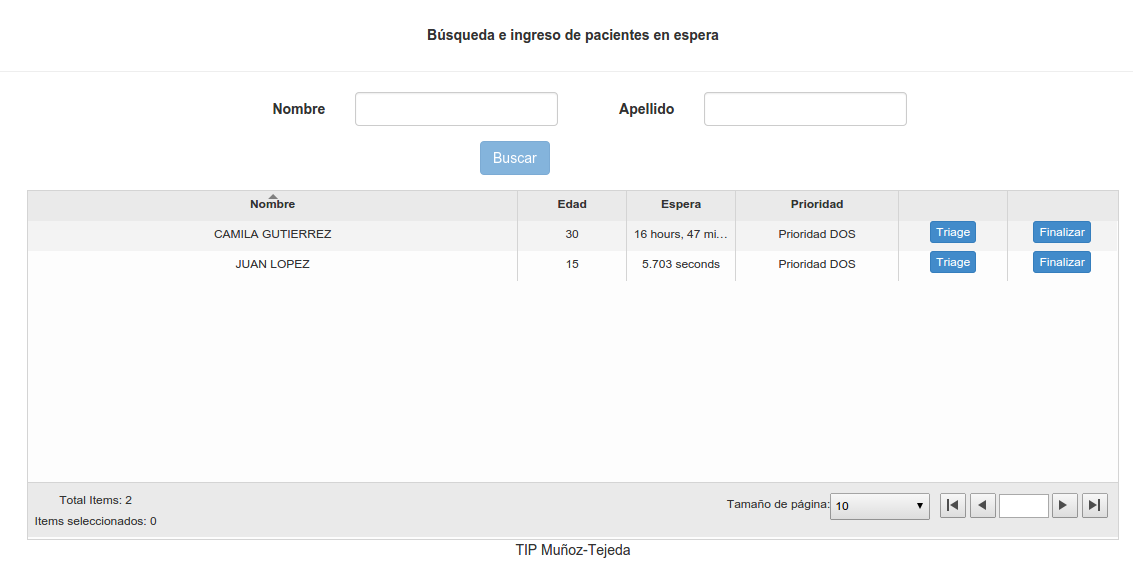
\includegraphics[width=0.99\textwidth]{espera.png}}
\caption{Lista de espera} \label{fig:espera}
\end{figure}
 La pantalla de lista de espera contiene un cuadro como los vistos anteriormente de personas así como los filtros para realizar búsquedas en ese cuadro. El cuadro muestra, también, el tiempo que ha pasado desde que el paciente ingresó a la guardia.

Esta pantalla es muy útil cuando la carga de síntomas es realizada por dos personas en ubicaciones físicas distinas. El paciente puede ser atendido en un mostrador (donde se toman sus síntomas, por ejemplo), y luego pasar a un consultorio para la toma de signos vitales. El enfermero en el consultorio debe solamente buscar al paciente en la lista de espera y podrá continuar grabando sus síntomas sin perder ninguna información ya cargada.

\subsection{Continuar el Triage}
En el caso de querer continuar el Triage de un paciente en lista de espera, el sistema permite buscar al paciente utilizando el filtro. Una vez localizado, a nivel fila del cuadro encontramos la opción ``Triage'' (figura \ref{fig:espera1})
\begin{figure}
\centerline{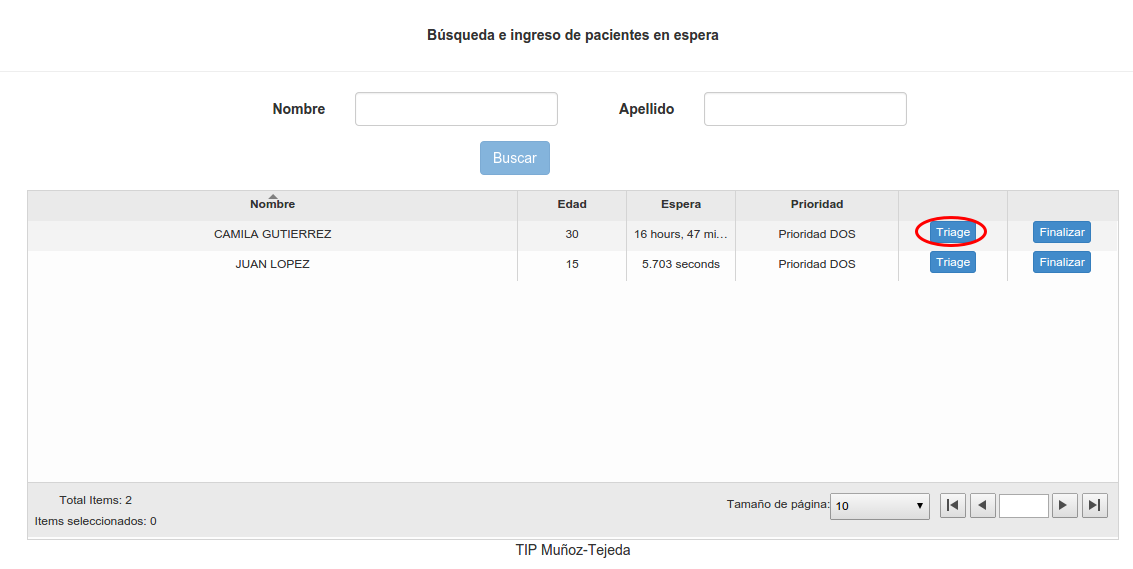
\includegraphics[width=0.99\textwidth]{espera1.png}}
\caption{Continuar el Triage} \label{fig:espera1}
\end{figure}
que permite volver a la pantalla de Triage del paciente seleccionado para continuar cargando síntomas o volver a calcular la prioridad.

\subsection{Finalizar}
Para finalizar el Triage, esto es, que el paciente salga del hospital o entre a consultorios/internación para recibir atención, el cuadro muestra, a nivel fila, la opción ``Finalizar'' (figura \ref{fig:espera2})
\begin{figure}
\centerline{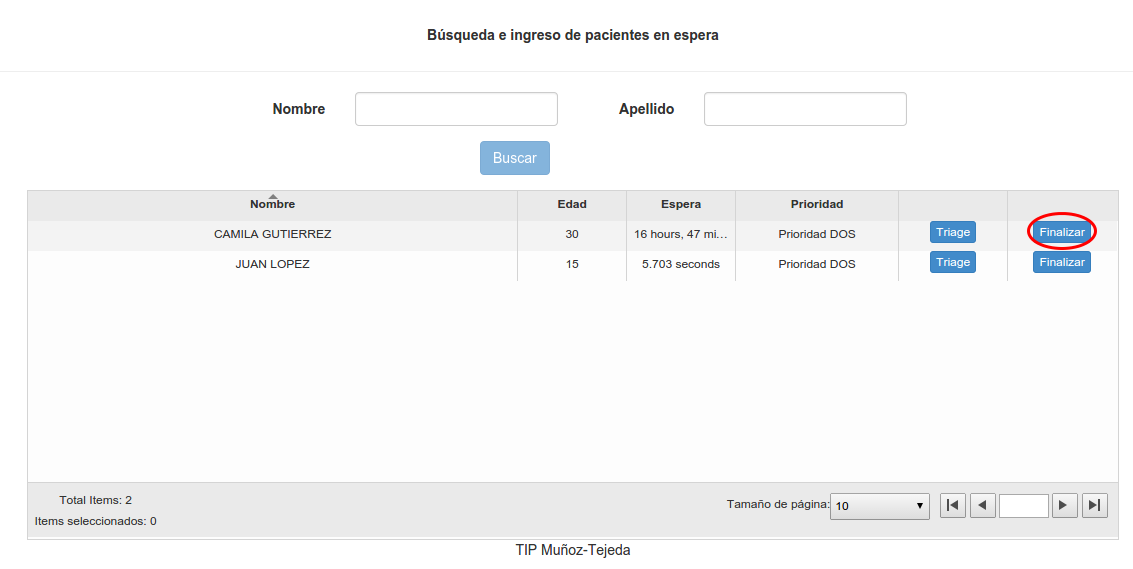
\includegraphics[width=0.99\textwidth]{espera2.png}}
\caption{Finalizar} \label{fig:espera2}
\end{figure}
que muestra una pantalla para indicar cuál fue la atención recibida por el paciente asi como sus datos y los síntomas cargados (figura \ref{fig:fin_atencion}).
\begin{figure}
\centerline{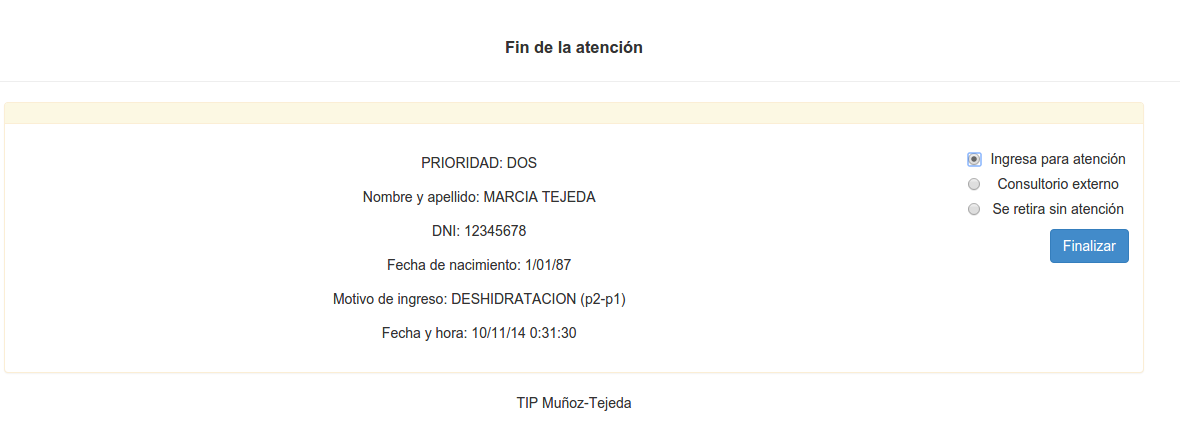
\includegraphics[width=0.99\textwidth]{fin_atencion.png}}
\caption{Fin de la atención} \label{fig:fin_atencion}
\end{figure}

Antes de finalizar la atención, el sistema guarda qué tipo de atención recibió el paciente, las cuales son:

\begin{itemize}
\item Ingresa para atención
\item Consultorio externo
\item Se retira sin atención
\end{itemize}